\subsection{Eksperimenta protokols: ORB OpenCV implementāciju ātrdarbība}\label{appx:test4}
\setcounter{table}{0} %Reset table counter for (sub)appendix
\setcounter{figure}{0} %Reset figure counter for (sub)appendix
Eksperimenta mērķis ir novērtēt OpenCV ORB algoritma implementācijas un
to variantu, tajā skaitā, tā OpenCL versijas (nejaukt ar OpenCV),
ātrdarbību dažādās ierīcēs.
Izmantotās ierīces atbilst iepriekšējo ekperimentu tabulās
\ref{tbl:test1-dev}~un \ref{tbl:test2-dev} uzrādītajām.

Par ieejas datiem tika izmantota ,,\termEn{bas-relief}'' attēlu kopa%
	\footnote{Pieejama no \url{http://www.edwardrosten.com/work/junk.tar}}
un visi konfigurējamie tika izmantoti visi noklusētie ORB algoritma parametri.
Katras attēla, iekārtas un implementācijas permutācijas tests tika atkārtots
30 reizes (kopā 1200 mērījumi). Rezultāti attēloti \ref{fig:test4-data}
attēlā, kur stabiņš atspoguļo zemāko no kopas attēlu apstrādes vidējiem
rādītājiem
(t.i., ,,grūtākā'' kopas attēla vidējais apstrādes ātrums 30 mērījumos).

\begin{figure}[tbh]
	\centering
	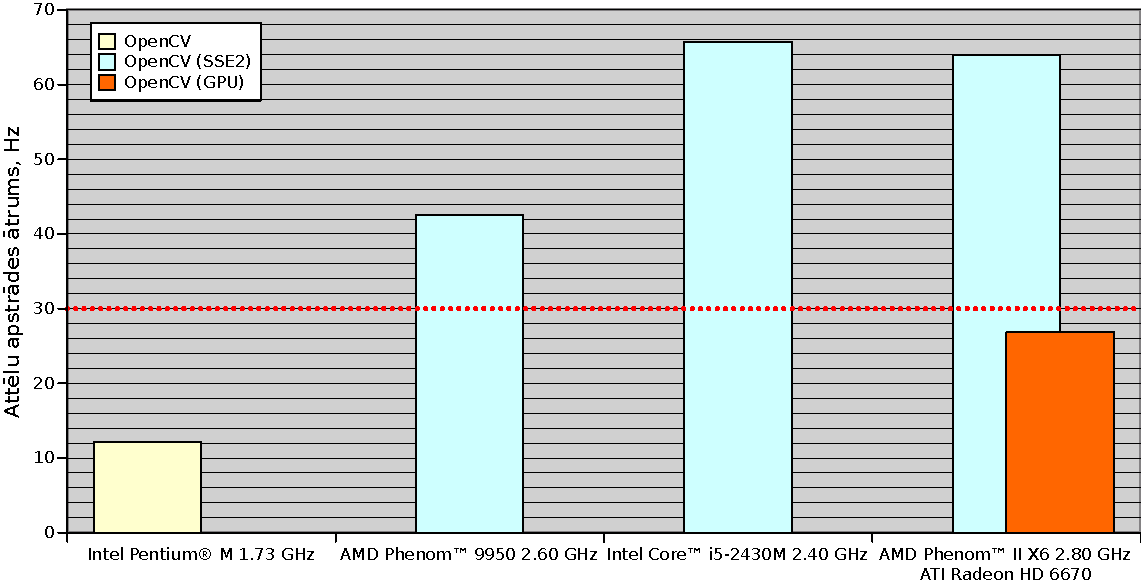
\includegraphics[width=\linewidth]{chart-orb}
	\caption{Ātrdarbība OpenCV ORB implementāciju variantiem dažādās ierīcēs.}
	\label{fig:test4-data}
\end{figure}

CPU implementācijas ātrdarbība atspoguļo izmantoto ierīču savstarpējo
skaitļošanas jaudas atšķirības līdzīgi FAST testiem, kas nav būtiski šajā
testā. Savukārt, interesants novērojums ir GPU implementācijas zemais
rezultāts --- mazāk kā puse no CPU (SSE2) implementācijas rādītāja, pat
nesasniedzot 30~kadru sekundē atzīmi.

Autors to skaidro ar nekorektu implementācijas modeli,
nevis platformas veiktspējas trūkumu, jo GPU implementācija sastāv no vairākām
apakšprogrammām, kuru katru izsaucot attēla dati atkārtoti jāpārvieto uz
GPU atmiņu.
%~ izmanto pārlieku augstu koda modularitāti ---
%~ FAST algoritms ir implementēts atsevišķi no ORB, un tiek izsaukts izpildot
%~ ORB. Tā ir pieņemta programmēšanas prakse CPU un neatstāj praktiski
%~ nekādu iespaidu uz ātrdarbību. Savukārt, izpildot neatkarīgas
%~ OpenCL apakšprogrammas GPU platformā, dati tiek lieki pārvietoti starp
%~ sistēmas operatīvo atmiņu un video atmiņu. Šajā gadījumā FAST noteikto
%~ raksturpunktu datu kopums tiek atgūts no video atmiņas un atkārtoti nosūtīts
%~ uz to izsaucot ORB. Pie tam pats ORB sastāv no vairākām OpenCL apakšprogrammām,
%~ kuras izsaucot jānosūta uz video atmiņu, kas, tādējādi, tiek izdarīts vairākas reizes.

%~ Autors arī konstatē, ka ORB OpenCL implementācija nerealizē Gausa filtrēšanu,
%~ bet to veic ar CPU. Gausa filtrēšanai ir augsts potenciāls ātrdarbības 
%~ uzlabošanai GPU un ņemot vērā, ka tā sastāda ievērojamu daļu ORB kopējā,
%~ kopējā implementācijas ātrdarbība tiek degradēta.

%~ Autors iesaka izveidot vienu OpenCL apakšprogrammu ORB izpildei, kas iekļauj
%~ %arī Gausa filtrēšanu un
%~ FAST raksturpunktu detektēšanu.
